\documentclass[11pt,aspectratio=169]{beamer}

\usepackage[T1]{fontenc}
\usepackage[utf8]{inputenc}
\usepackage{lmodern}
\usepackage{microtype}
\usepackage{graphicx}
\usepackage{booktabs}
\usepackage{tabularx}
\usepackage{array}
\usepackage{tikz}
\usetikzlibrary{arrows.meta,positioning}
\usepackage{ragged2e}

\usetheme{default}
\setbeamertemplate{navigation symbols}{}
\setbeamertemplate{footline}[frame number]
\setbeamersize{text margin left=0.75cm,text margin right=0.75cm}

\definecolor{Primary}{HTML}{17324D}
\definecolor{Accent}{HTML}{1F7A8C}
\definecolor{Gold}{HTML}{C68A2F}
\definecolor{SoftBlue}{HTML}{EAF3F7}
\definecolor{SoftGreen}{HTML}{EAF4EC}
\definecolor{SoftGold}{HTML}{FBF3E3}
\definecolor{SoftRed}{HTML}{FBEAEC}
\definecolor{TextGray}{HTML}{4E5B67}
\definecolor{LineGray}{HTML}{D6DEE4}

\setbeamercolor{background canvas}{bg=white}
\setbeamercolor{normal text}{fg=Primary,bg=white}
\setbeamercolor{title}{fg=Primary}
\setbeamercolor{frametitle}{fg=Primary}
\setbeamercolor{subtitle}{fg=TextGray}
\setbeamercolor{block title}{fg=white,bg=Accent}
\setbeamercolor{block body}{fg=Primary,bg=SoftBlue}
\setbeamercolor{alertblock title}{fg=white,bg=Gold}
\setbeamercolor{alertblock body}{fg=Primary,bg=SoftGold}
\setbeamercolor{exampleblock title}{fg=white,bg=Accent!80!black}
\setbeamercolor{exampleblock body}{fg=Primary,bg=SoftGreen}

\setbeamerfont{title}{series=\bfseries,size=\LARGE}
\setbeamerfont{frametitle}{series=\bfseries,size=\Large}
\setbeamerfont{subtitle}{size=\large}
\setbeamerfont{block title}{series=\bfseries}

\setbeamertemplate{itemize item}{\color{Accent}$\blacktriangleright$}
\setbeamertemplate{itemize subitem}{\color{Gold}$\bullet$}

\newcommand{\PresenterName}{[Presenter Name]}
\newcommand{\TeamName}{[Team or Group]}
\newcommand{\CourseName}{[Course / Internal Handoff]}
\newcommand{\ShowcaseImage}{assets/showcase.png}

\newcommand{\KeyMessage}[1]{%
  \begin{beamercolorbox}[wd=\linewidth,rounded=true,sep=8pt]{block body}
    \centering\bfseries #1
  \end{beamercolorbox}
}

\newcommand{\MiniCard}[3]{%
  \begin{beamercolorbox}[wd=\linewidth,rounded=true,sep=8pt]{#1}
    {\bfseries #2}\par
    \vspace{2pt}
    #3
  \end{beamercolorbox}
}

\newcommand{\PhaseBadge}[1]{%
  \tikz[baseline=(node.base)] \node[
    fill=Accent,
    text=white,
    rounded corners=2pt,
    inner xsep=5pt,
    inner ysep=2pt,
    font=\bfseries\small
  ] (node) {#1};
}

\newcommand{\RoadmapRow}[3]{%
  \PhaseBadge{#1} & \textbf{#2} & #3 \\
}

\title{Connections Puzzle Generator}
\subtitle{System Scaffold, Quality-Control Plan, and Implementation Handoff}
\author{\PresenterName}
\institute{\TeamName \textbar{} \CourseName}
\date{\today}

\begin{document}

% Slide 1 -----------------------------------------------------------
\begin{frame}[plain]
  \begin{columns}[c,onlytextwidth]
    \begin{column}{0.56\textwidth}
      {\usebeamerfont{title}\inserttitle\par}
      \vspace{0.2cm}
      {\usebeamerfont{subtitle}\insertsubtitle\par}
      \vspace{0.35cm}

      \KeyMessage{A production-style system for generating, evaluating, and debugging NYT-Connections-style puzzles.}

      \vspace{0.45cm}
      \begin{itemize}
        \item End-to-end demo mode already runs.
        \item Quality-control infrastructure is scaffolded.
        \item Puzzle-quality heuristics remain intentionally human-owned.
      \end{itemize}

      \vfill
      {\small \textbf{Presenter:} \PresenterName \hspace{0.5cm}
      \textbf{Team:} \TeamName \hspace{0.5cm}
      \textbf{Context:} \CourseName}
    \end{column}
    \begin{column}{0.40\textwidth}
      \IfFileExists{\ShowcaseImage}{
        \includegraphics[width=\linewidth]{\ShowcaseImage}
      }{
        \fbox{\parbox[c][0.55\textheight][c]{0.95\linewidth}{\centering
          Showcase image placeholder\\
          \vspace{4pt}
          \texttt{assets/showcase.png}}}
      }
    \end{column}
  \end{columns}
\end{frame}

% Slide 2 -----------------------------------------------------------
\begin{frame}{What This Project Is}
  \begin{columns}[T,onlytextwidth]
    \begin{column}{0.48\textwidth}
      \begin{block}{Puzzle Format}
        \begin{itemize}
          \item 16 words
          \item Partitioned into 4 groups of 4
          \item Each group has an internal connection
        \end{itemize}
      \end{block}
    \end{column}
    \begin{column}{0.48\textwidth}
      \begin{block}{Our Task}
        \begin{itemize}
          \item Generate puzzles
          \item Not just solve or classify them
          \item Produce puzzles that survive quality control
        \end{itemize}
      \end{block}
    \end{column}
  \end{columns}

  \vspace{0.25cm}
  \begin{alertblock}{Why Generation Is Hard}
    Good local groups are not enough; the whole puzzle must avoid multiple plausible solutions.
  \end{alertblock}
\end{frame}

% Slide 3 -----------------------------------------------------------
\begin{frame}{Current Product Status}
  \begin{columns}[T,onlytextwidth]
    \begin{column}{0.32\textwidth}
      \MiniCard{exampleblock body}{Frontend Surface}{
        React + TypeScript + Vite\\
        Puzzle board, reveal panel, score panel, debug view
      }
    \end{column}
    \begin{column}{0.32\textwidth}
      \MiniCard{block body}{Backend + Pipeline}{
        FastAPI, typed schemas, services, demo generation, trace metadata
      }
    \end{column}
    \begin{column}{0.32\textwidth}
      \MiniCard{alertblock body}{Evaluation + Debug}{
        Batch evaluation, accepted/rejected persistence, top-k browsing
      }
    \end{column}
  \end{columns}

  \vspace{0.45cm}
  \KeyMessage{This repo is already a real product scaffold, not just disconnected code fragments.}
\end{frame}

% Slide 4 -----------------------------------------------------------
\begin{frame}{Demo and Product Surfaces}
  \begin{columns}[T,onlytextwidth]
    \begin{column}{0.56\textwidth}
      \IfFileExists{\ShowcaseImage}{
        \includegraphics[width=\linewidth]{\ShowcaseImage}
      }{
        \fbox{\parbox[c][0.46\textheight][c]{0.95\linewidth}{\centering
          UI showcase placeholder}}
      }
    \end{column}
    \begin{column}{0.40\textwidth}
      \begin{block}{What the UI Already Exposes}
        \begin{itemize}
          \item Generate Puzzle
          \item Load Static Sample
          \item Reveal Answers
          \item Developer Mode
          \item Top-K / batch debug summary
        \end{itemize}
      \end{block}

      \vspace{0.15cm}
      \begin{exampleblock}{Demo Message}
        We can show both the product-facing flow and the engineering-facing debug flow in one interface.
      \end{exampleblock}
    \end{column}
  \end{columns}
\end{frame}

% Slide 5 -----------------------------------------------------------
\begin{frame}{Big-Picture Architecture}
  \centering
  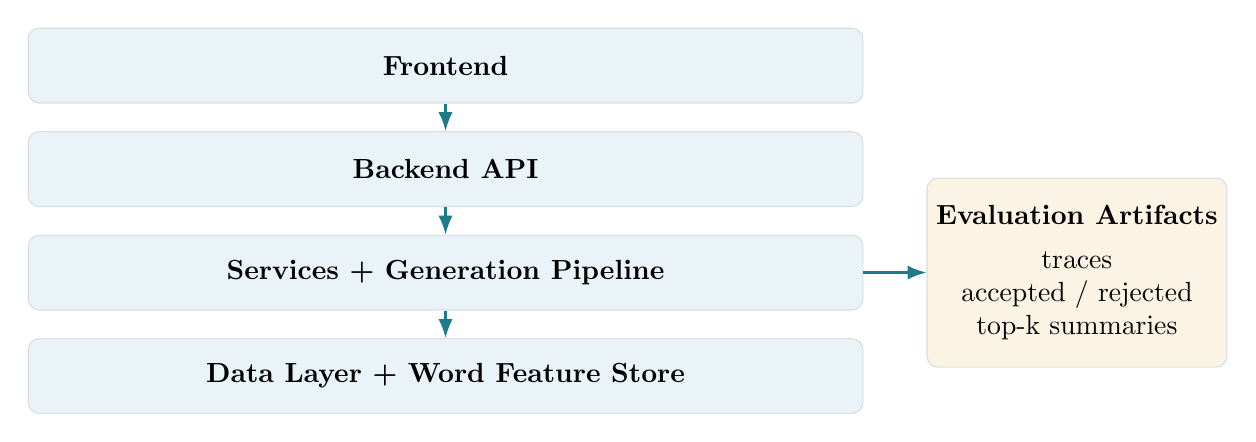
\begin{tikzpicture}[
    node distance=0.35cm,
    layer/.style={
      rounded corners=4pt,
      minimum width=10.6cm,
      minimum height=0.95cm,
      draw=LineGray,
      fill=SoftBlue,
      align=center,
      font=\bfseries
    },
    sidebox/.style={
      rounded corners=4pt,
      minimum width=3.1cm,
      minimum height=2.4cm,
      draw=LineGray,
      fill=SoftGold,
      align=center
    },
    flow/.style={-{Latex[length=2.4mm]}, draw=Accent, thick}
  ]
    \node[layer] (frontend) {Frontend};
    \node[layer, below=of frontend] (api) {Backend API};
    \node[layer, below=of api] (services) {Services + Generation Pipeline};
    \node[layer, below=of services] (data) {Data Layer + Word Feature Store};
    \node[sidebox, right=0.8cm of services] (artifacts) {\textbf{Evaluation Artifacts}\\[4pt]
      traces\\
      accepted / rejected\\
      top-k summaries};

    \draw[flow] (frontend) -- (api);
    \draw[flow] (api) -- (services);
    \draw[flow] (services) -- (data);
    \draw[flow] (services.east) -- (artifacts.west);
  \end{tikzpicture}

  \vspace{0.35cm}
  \KeyMessage{Frontend on top, pipeline in the middle,\\ reusable data and evaluation artifacts underneath.}
\end{frame}

% Slide 6 -----------------------------------------------------------
\begin{frame}{Main Generation Pipeline}
  \textbf{1. Build a candidate}
  \begin{center}
    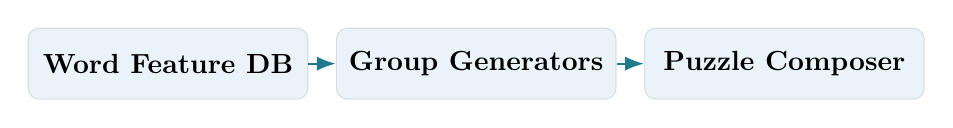
\begin{tikzpicture}[
      box/.style={
        rounded corners=4pt,
        minimum width=3.55cm,
        minimum height=0.9cm,
        draw=LineGray,
        fill=SoftBlue,
        align=center
      },
      flow/.style={-{Latex[length=2.4mm]}, draw=Accent, thick},
      node distance=0.35cm
    ]
      \node[box] (db) {\textbf{Word Feature DB}};
      \node[box, right=of db] (gen) {\textbf{Group Generators}};
      \node[box, right=of gen] (comp) {\textbf{Puzzle Composer}};
      \draw[flow] (db) -- (gen);
      \draw[flow] (gen) -- (comp);
    \end{tikzpicture}
  \end{center}

  \vspace{0.25cm}
  \textbf{2. Judge the candidate}
  \begin{center}
    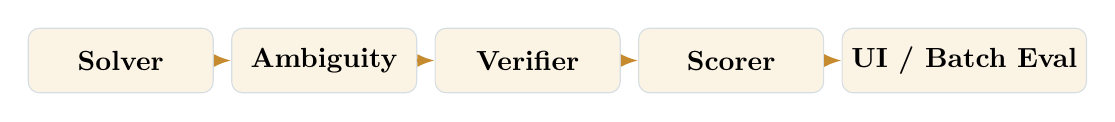
\begin{tikzpicture}[
      box/.style={
        rounded corners=4pt,
        minimum width=2.35cm,
        minimum height=0.82cm,
        draw=LineGray,
        fill=SoftGold,
        align=center
      },
      flow/.style={-{Latex[length=2.2mm]}, draw=Gold, thick},
      node distance=0.22cm
    ]
      \node[box] (solver) {\textbf{Solver}};
      \node[box, right=of solver] (ambiguity) {\textbf{Ambiguity}};
      \node[box, right=of ambiguity] (verifier) {\textbf{Verifier}};
      \node[box, right=of verifier] (scorer) {\textbf{Scorer}};
      \node[box, right=of scorer] (outputs) {\textbf{UI / Batch Eval}};
      \draw[flow] (solver) -- (ambiguity);
      \draw[flow] (ambiguity) -- (verifier);
      \draw[flow] (verifier) -- (scorer);
      \draw[flow] (scorer) -- (outputs);
    \end{tikzpicture}
  \end{center}

  \vspace{0.12cm}
  \KeyMessage{The project is not just a generator; it is a generator plus a quality-control pipeline.}
\end{frame}

% Slide 7 -----------------------------------------------------------
\begin{frame}{Four Generator Families}
  \begin{columns}[T,onlytextwidth]
    \begin{column}{0.48\textwidth}
      \begin{block}{Semantic}
        Main stable generator.\\
        Best first target for strong, reliable groups.
      \end{block}

      \vspace{0.18cm}
      \begin{block}{Lexical}
        Pattern and template diversity.\\
        Helps avoid every puzzle feeling semantically uniform.
      \end{block}
    \end{column}
    \begin{column}{0.48\textwidth}
      \begin{block}{Theme}
        NYT-like thematic richness.\\
        Important for memorable, human-feeling puzzles.
      \end{block}

      \vspace{0.18cm}
      \begin{block}{Phonetic / Wordplay}
        High-upside category for cleverness.\\
        Also the hardest and most later-stage generator.
      \end{block}
    \end{column}
  \end{columns}
\end{frame}

% Slide 8 -----------------------------------------------------------
\begin{frame}{Why Quality Control Matters}
  \begin{columns}[T,onlytextwidth]
    \begin{column}{0.47\textwidth}
      \begin{exampleblock}{What Generation Can Get Right}
        \begin{itemize}
          \item Each group looks internally coherent
          \item The categories feel individually plausible
          \item The final 16 words look interesting
        \end{itemize}
      \end{exampleblock}
    \end{column}
    \begin{column}{0.47\textwidth}
      \begin{alertblock}{What Can Still Go Wrong}
        \begin{itemize}
          \item Words leak across groups
          \item Multiple plausible partitions exist
          \item The puzzle is technically valid but stylistically weak
        \end{itemize}
      \end{alertblock}
    \end{column}
  \end{columns}

  \vspace{0.25cm}
  \KeyMessage{Generating categories is only half the problem; the real challenge is controlling ambiguity at the full-puzzle level.}
\end{frame}

% Slide 9 -----------------------------------------------------------
\begin{frame}{Ambiguity Evaluator, Verifier, and Scorer}
  \begin{columns}[T,onlytextwidth]
    \begin{column}{0.31\textwidth}
      \begin{block}{Ambiguity Evaluator}
        \textbf{Goal:} inspect structural risk.\\[4pt]
        \textbf{Output:} leakage evidence, alternative grouping candidates, risk level.
      \end{block}
    \end{column}
    \begin{column}{0.31\textwidth}
      \begin{alertblock}{Verifier}
        \textbf{Goal:} act as the hard gate.\\[4pt]
        \textbf{Output:} accept, reject, or borderline with explicit reasons.
      \end{alertblock}
    \end{column}
    \begin{column}{0.31\textwidth}
      \begin{exampleblock}{Scorer}
        \textbf{Goal:} rank what survives.\\[4pt]
        \textbf{Output:} coherence, ambiguity penalties, style metadata, overall score.
      \end{exampleblock}
    \end{column}
  \end{columns}

  \vspace{0.2cm}
  \KeyMessage{These modules do different jobs: evidence, gating, and ranking should not be collapsed into one heuristic blob.}
\end{frame}

% Slide 10 ----------------------------------------------------------
\begin{frame}{Second-Stage Scaffold Already Completed}
  \begin{block}{What the repo already supports today}
    \begin{tabularx}{\linewidth}{>{\bfseries}p{3.2cm} X}
      Solver ensemble & Multiple solver adapters, per-solver votes, agreement/disagreement summaries \\
      \addlinespace[4pt]
      Ambiguity scaffold & Structured leakage evidence, alternative grouping records, risk reports \\
      \addlinespace[4pt]
      Style-analysis scaffold & Placeholder style signals, archetype labels, transparent non-final reporting \\
      \addlinespace[4pt]
      Batch evaluation & Offline runs, accepted/rejected persistence, summary metrics, saved top-k outputs \\
      \addlinespace[4pt]
      Top-k debug & Developer-facing browsing for best accepted puzzles and comparison metadata \\
    \end{tabularx}
  \end{block}

  \vspace{0.12cm}
  \begin{alertblock}{Important boundary}
    The infrastructure exists. The true puzzle-quality heuristics do not.
  \end{alertblock}
\end{frame}

% Slide 11 ----------------------------------------------------------
\begin{frame}{Implemented Scaffold vs Human-Owned Core Logic}
  \begin{columns}[T,onlytextwidth]
    \begin{column}{0.48\textwidth}
      \begin{exampleblock}{Already Implemented}
        \begin{itemize}
          \item FastAPI backend and React frontend
          \item Demo generation pipeline
          \item Typed schemas and trace metadata
          \item Solver registry and ensemble scaffold
          \item Ambiguity, style, batch-eval, and top-k scaffolds
        \end{itemize}
      \end{exampleblock}
    \end{column}
    \begin{column}{0.48\textwidth}
      \begin{alertblock}{Still Intentionally Human-Owned}
        \begin{itemize}
          \item High-quality feature engineering
          \item Real generator quality for all four families
          \item Leakage reasoning and alternative partition search
          \item Final verifier policy and score calibration
          \item Real NYT-likeness and style judgment
        \end{itemize}
      \end{alertblock}
    \end{column}
  \end{columns}
\end{frame}

% Slide 12 ----------------------------------------------------------
\begin{frame}{Implementation Roadmap}
  \begin{block}{Recommended order of execution}
    \begin{tabularx}{\linewidth}{>{\raggedright\arraybackslash}p{1.6cm} >{\raggedright\arraybackslash}p{3.2cm} X}
      \RoadmapRow{Phase 1}{Representation + generation core}{Semantic feature DB, semantic generator, and puzzle composer}
      \RoadmapRow{Phase 2}{Quality gate}{Ambiguity evaluator, verifier, and scorer}
      \RoadmapRow{Phase 3}{Diversity}{Lexical generator and theme generator}
      \RoadmapRow{Phase 4}{Tuning loop}{Batch evaluation, analysis, and acceptance tuning}
      \RoadmapRow{Phase 5}{A+ layer}{Phonetic generator, style calibration, final polish}
    \end{tabularx}
  \end{block}

  \vspace{0.2cm}
  \KeyMessage{Build the stable semantic core first; add richer diversity and polish only after the quality gate exists.}
\end{frame}

% Slide 13 ----------------------------------------------------------
\begin{frame}{MVP vs Strong Version vs A+ Enhancements}
  \begin{columns}[T,onlytextwidth]
    \begin{column}{0.31\textwidth}
      \begin{block}{MVP}
        \begin{itemize}
          \item Semantic feature DB
          \item Semantic generator
          \item Composer
          \item Ambiguity + verifier + scorer
          \item Batch eval + web UI
        \end{itemize}
      \end{block}
    \end{column}
    \begin{column}{0.31\textwidth}
      \begin{exampleblock}{Strong Version}
        \begin{itemize}
          \item Better semantic coverage
          \item Better composer constraints
          \item More reliable ranking
          \item Stronger tuning loop
        \end{itemize}
      \end{exampleblock}
    \end{column}
    \begin{column}{0.31\textwidth}
      \begin{alertblock}{A+ Enhancements}
        \begin{itemize}
          \item Theme depth
          \item Phonetic / wordplay groups
          \item Historical style calibration
          \item Better solver ensemble and UI polish
        \end{itemize}
      \end{alertblock}
    \end{column}
  \end{columns}
\end{frame}

% Slide 14 ----------------------------------------------------------
\begin{frame}{Team Action Slide: What Must Be Owned Next}
  \begin{columns}[T,onlytextwidth]
    \begin{column}{0.48\textwidth}
      \begin{block}{Core build work}
        \begin{itemize}
          \item Feature extraction: define semantic, lexical, phonetic, and theme-oriented signals
          \item Generator quality: make semantic strong first, then add lexical and theme diversity
          \item Composer: enforce deduplication, compatibility, and puzzle-level rules
          \item Ambiguity: turn scaffolded evidence into real leakage reasoning and regrouping search
        \end{itemize}
      \end{block}
    \end{column}
    \begin{column}{0.48\textwidth}
      \begin{exampleblock}{Quality gate and tuning}
        \begin{itemize}
          \item Verifier: define the accept / reject / borderline policy clearly
          \item Scorer: rank accepted puzzles with calibrated, explainable signals
          \item Evaluation and calibration: use batch runs, top-k review, and traces to improve quality over time
        \end{itemize}
      \end{exampleblock}
    \end{column}
  \end{columns}
\end{frame}

% Slide 15 ----------------------------------------------------------
\begin{frame}{Closing Takeaway}
  \begin{block}{Why this project is compelling}
    \begin{itemize}
      \item It already has a credible product surface and engineering scaffold.
      \item It is honest about what is solved and what is not.
      \item The remaining work is meaningful research-engineering, not basic plumbing.
    \end{itemize}
  \end{block}

  \vspace{0.25cm}
  \KeyMessage{The scaffold is ready; the next step is to turn human-owned judgment into measurable puzzle quality.}
\end{frame}

\end{document}
